\begin{figure}[h!]
    \centering{
        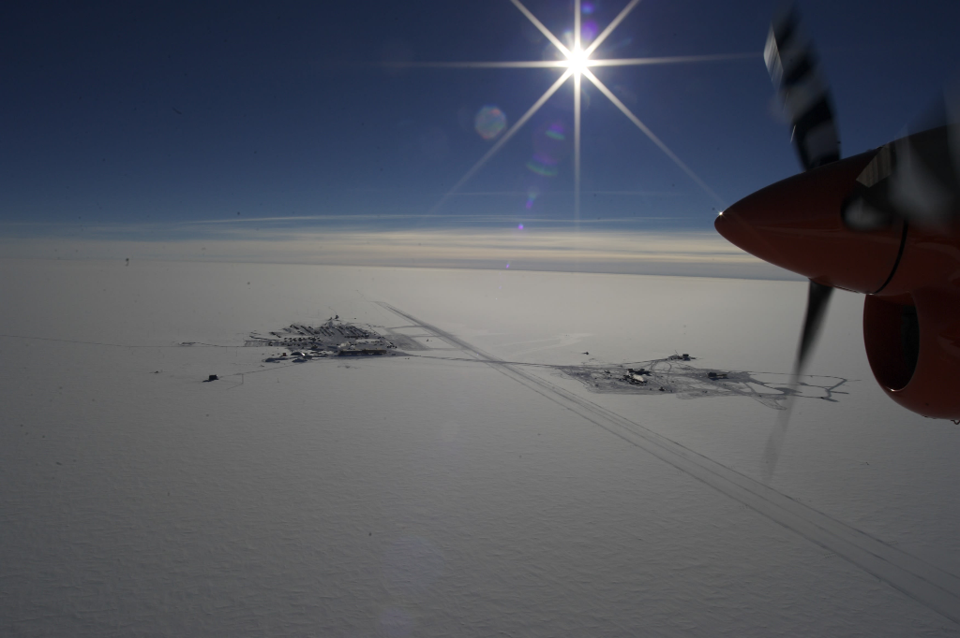
\includegraphics[clip, trim=3cm 3.5cm 2cm 0cm, scale=0.8]{figures/ic3/IC3_aboveground.png}
    }
    \caption{IceCube Neutrino observatory and science center at the South Pole. Detector volume is beneath glacial ice. Image from \cite{IceCube_SPGallery}.}
    \label{fig:IC3_atPole}
\end{figure}

Located at the South Pole, the IceCube Neutrino Observatory is a pivotal instrument for neutrino astronomy.
The above and below ice components of the IceCube observatory are shown in \cref{fig:IC3_atPole,fig:IC3_full_detector}.
IceCube's primary function is the detection and analysis of elusive, high-energy neutrinos.
These neutrinos carry information from the most energetic and distant cosmic phenomena.
The observatory uses thousands of digital optical modules embedded in a cubic kilometer of Antarctic ice to detect Cherenkov radiation.
This radiation occurs when neutrinos interact with the ice, revealing their origin and energy.

IceCube is a critical component in the multi-messenger astrophysics toolkit, especially in the search for dark matter and beyond standard model (BSM) astrophysical processes.
The observatory's analysis of neutrino signals enhances our understanding of the universe by correlating these signals with other cosmic messengers, including electromagnetic, gravitational waves, and cosmic rays.
The following sections will discuss the observatory's design, data acquisition, and event reconstruction methodologies.

%-----------------------------------------------------------------------------------%
\section{The Detector}
%-----------------------------------------------------------------------------------%

\begin{figure}
    \centering{
        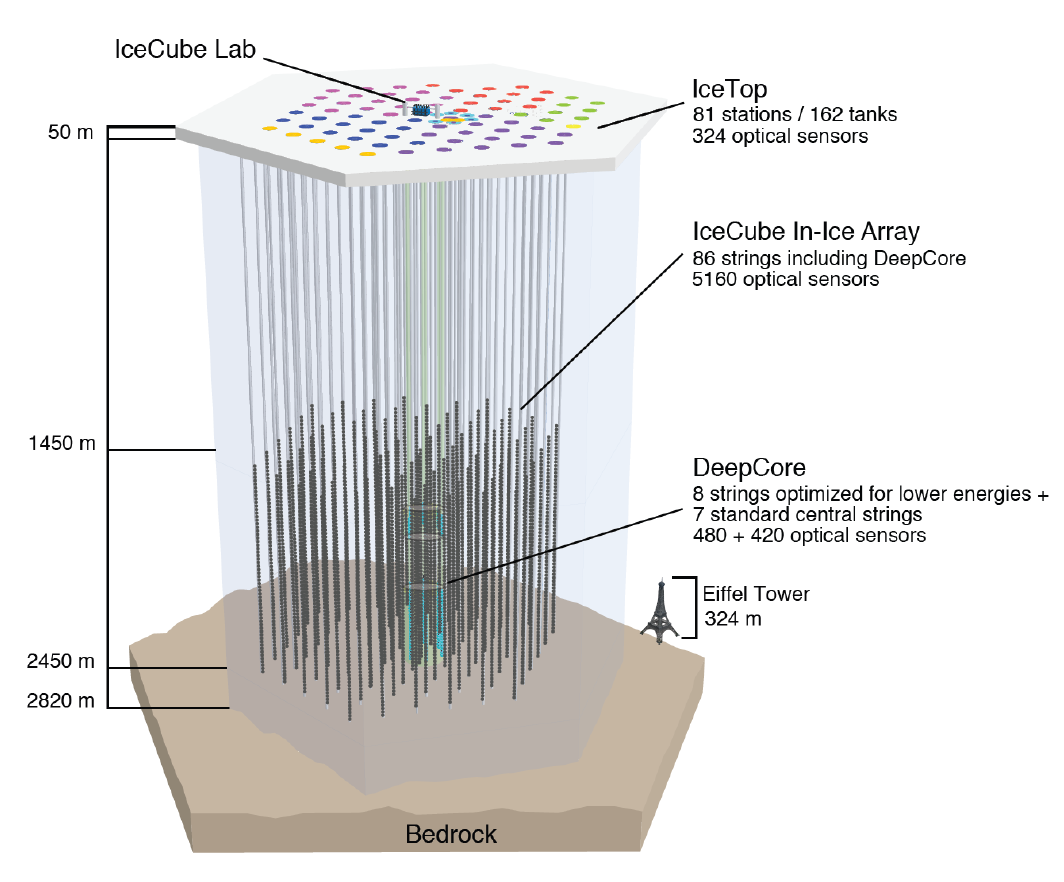
\includegraphics[scale=0.5]{figures/ic3/icecube.png}
    }
    \caption{Graphic of the full IceCube Neutrino Observatory. In-ice array is made up of 86 strings with a total of 5160 optical sensors. Deepcore is a denser arrangement of optical sensors for sensitivity to lower energy neutrinos. Figure from \cite{IceCube_SPGallery}.}
    \label{fig:IC3_full_detector}
\end{figure}

The IceCube Neutrino Observatory is embedded within a cubic kilometer of Antarctic ice at the South Pole.
IceCube's modules are designed to detect neutrinos through Cherenkov radiation emitted after neutrino interactions within the ice.
It comprises of 5160 Digital Optical Modules (DOMs), arranged across 86 strings that span depths of 1450 m to 2450 m beneath the surface.
This arrangement allows IceCube to capture high-energy neutrinos across a broad neutrino energy spectrum.

%$$$$$$$$$$$$$$$$$$$$$$$$$$$$$$$$$$$$$$$$$$$$$$$$$$$$$$$$$$$$$$$$$$$$$$$$$$$$$$$$$$$%
\subsection{Hardware and Construction}
%$$$$$$$$$$$$$$$$$$$$$$$$$$$$$$$$$$$$$$$$$$$$$$$$$$$$$$$$$$$$$$$$$$$$$$$$$$$$$$$$$$$%

\begin{figure}
    \centering{
        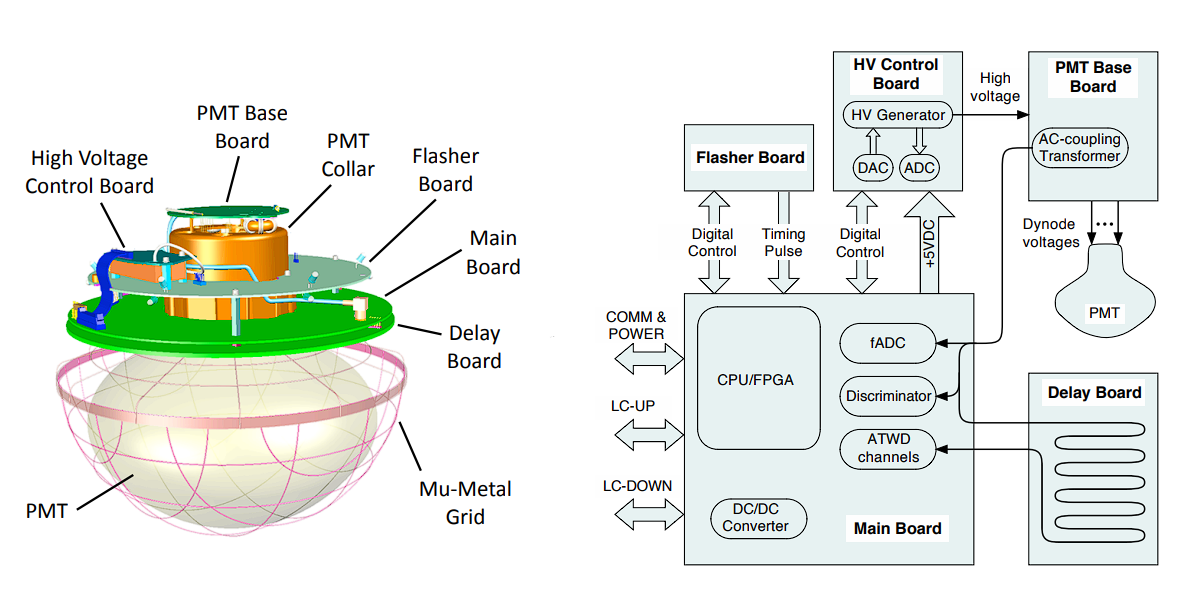
\includegraphics[scale=0.5]{figures/ic3/DOM.png}
    }
    \caption{Composition of the Digital Optical Module (DOM). Left image is an illustration of the mechanical layout. Right is a flow chart of functional connections. Figure from \cite{IC3_thedetector}}
    \label{fig:DOM}
\end{figure}

Digital Optical Modules (DOMs) are at the core of IceCube’s detection technology.
\Cref{fig:DOM} illustrates the construction and signal flow of a DOM.
Each DOM is encased in a glass sphere that can withstand deep-ice pressures.
A DOM features a 10-inch PMT for Cherenkov light detection, a high-voltage power supply for the PMT, and a Main Board for signal digitization and timestamping.
An LED Flasher Board is included for calibration purposes.
They assist in verifying DOM responses and measuring the glacial ice's optical properties.
The DOMs are deployed along cables on strings in a hexagonal grid pattern that spans a cubic kilometer.
Strings are placed with 125 m of horizontal spacing, and DOMs are vertically separated by 17 m on each string.
This detector geometry optimizes detection of TeV to PeV neutrinos.

DeepCore and IceTop, additional components of IceCube, extend its research capabilities.
DeepCore, with its denser array of DOMs, targets lower energy neutrinos for studies such as neutrino oscillations.
IceTop, situated at the ice surface, measures cosmic rays, contributing data that complement the neutrino observations from below the ice.
\Cref{fig:IC3_full_detector} illustrates the full detector volume and auxiliary systems.

The central hub for IceCube's operations is the IceCube Laboratory (ICL) and is situated at the surface at the center of the array (see \cref{fig:ICL}).
This facility houses the servers and computers responsible for data acquisition and online filtering.
ICL connects to the DOMs via cables routed up from beneath the ice \cite{IC3_thedetector}.
The ICL manages the data flow from the ice, ensuring continuous operation and data integrity.
It maintains optimal conditions for its electronic equipment, including temperature control and protection against electromagnetic interference \cite{IC3_thedetector}.


%$$$$$$$$$$$$$$$$$$$$$$$$$$$$$$$$$$$$$$$$$$$$$$$$$$$$$$$$$$$$$$$$$$$$$$$$$$$$$$$$$$$%
\subsection{Data Acquisition}
%$$$$$$$$$$$$$$$$$$$$$$$$$$$$$$$$$$$$$$$$$$$$$$$$$$$$$$$$$$$$$$$$$$$$$$$$$$$$$$$$$$$%

\begin{figure}
    \centering{
        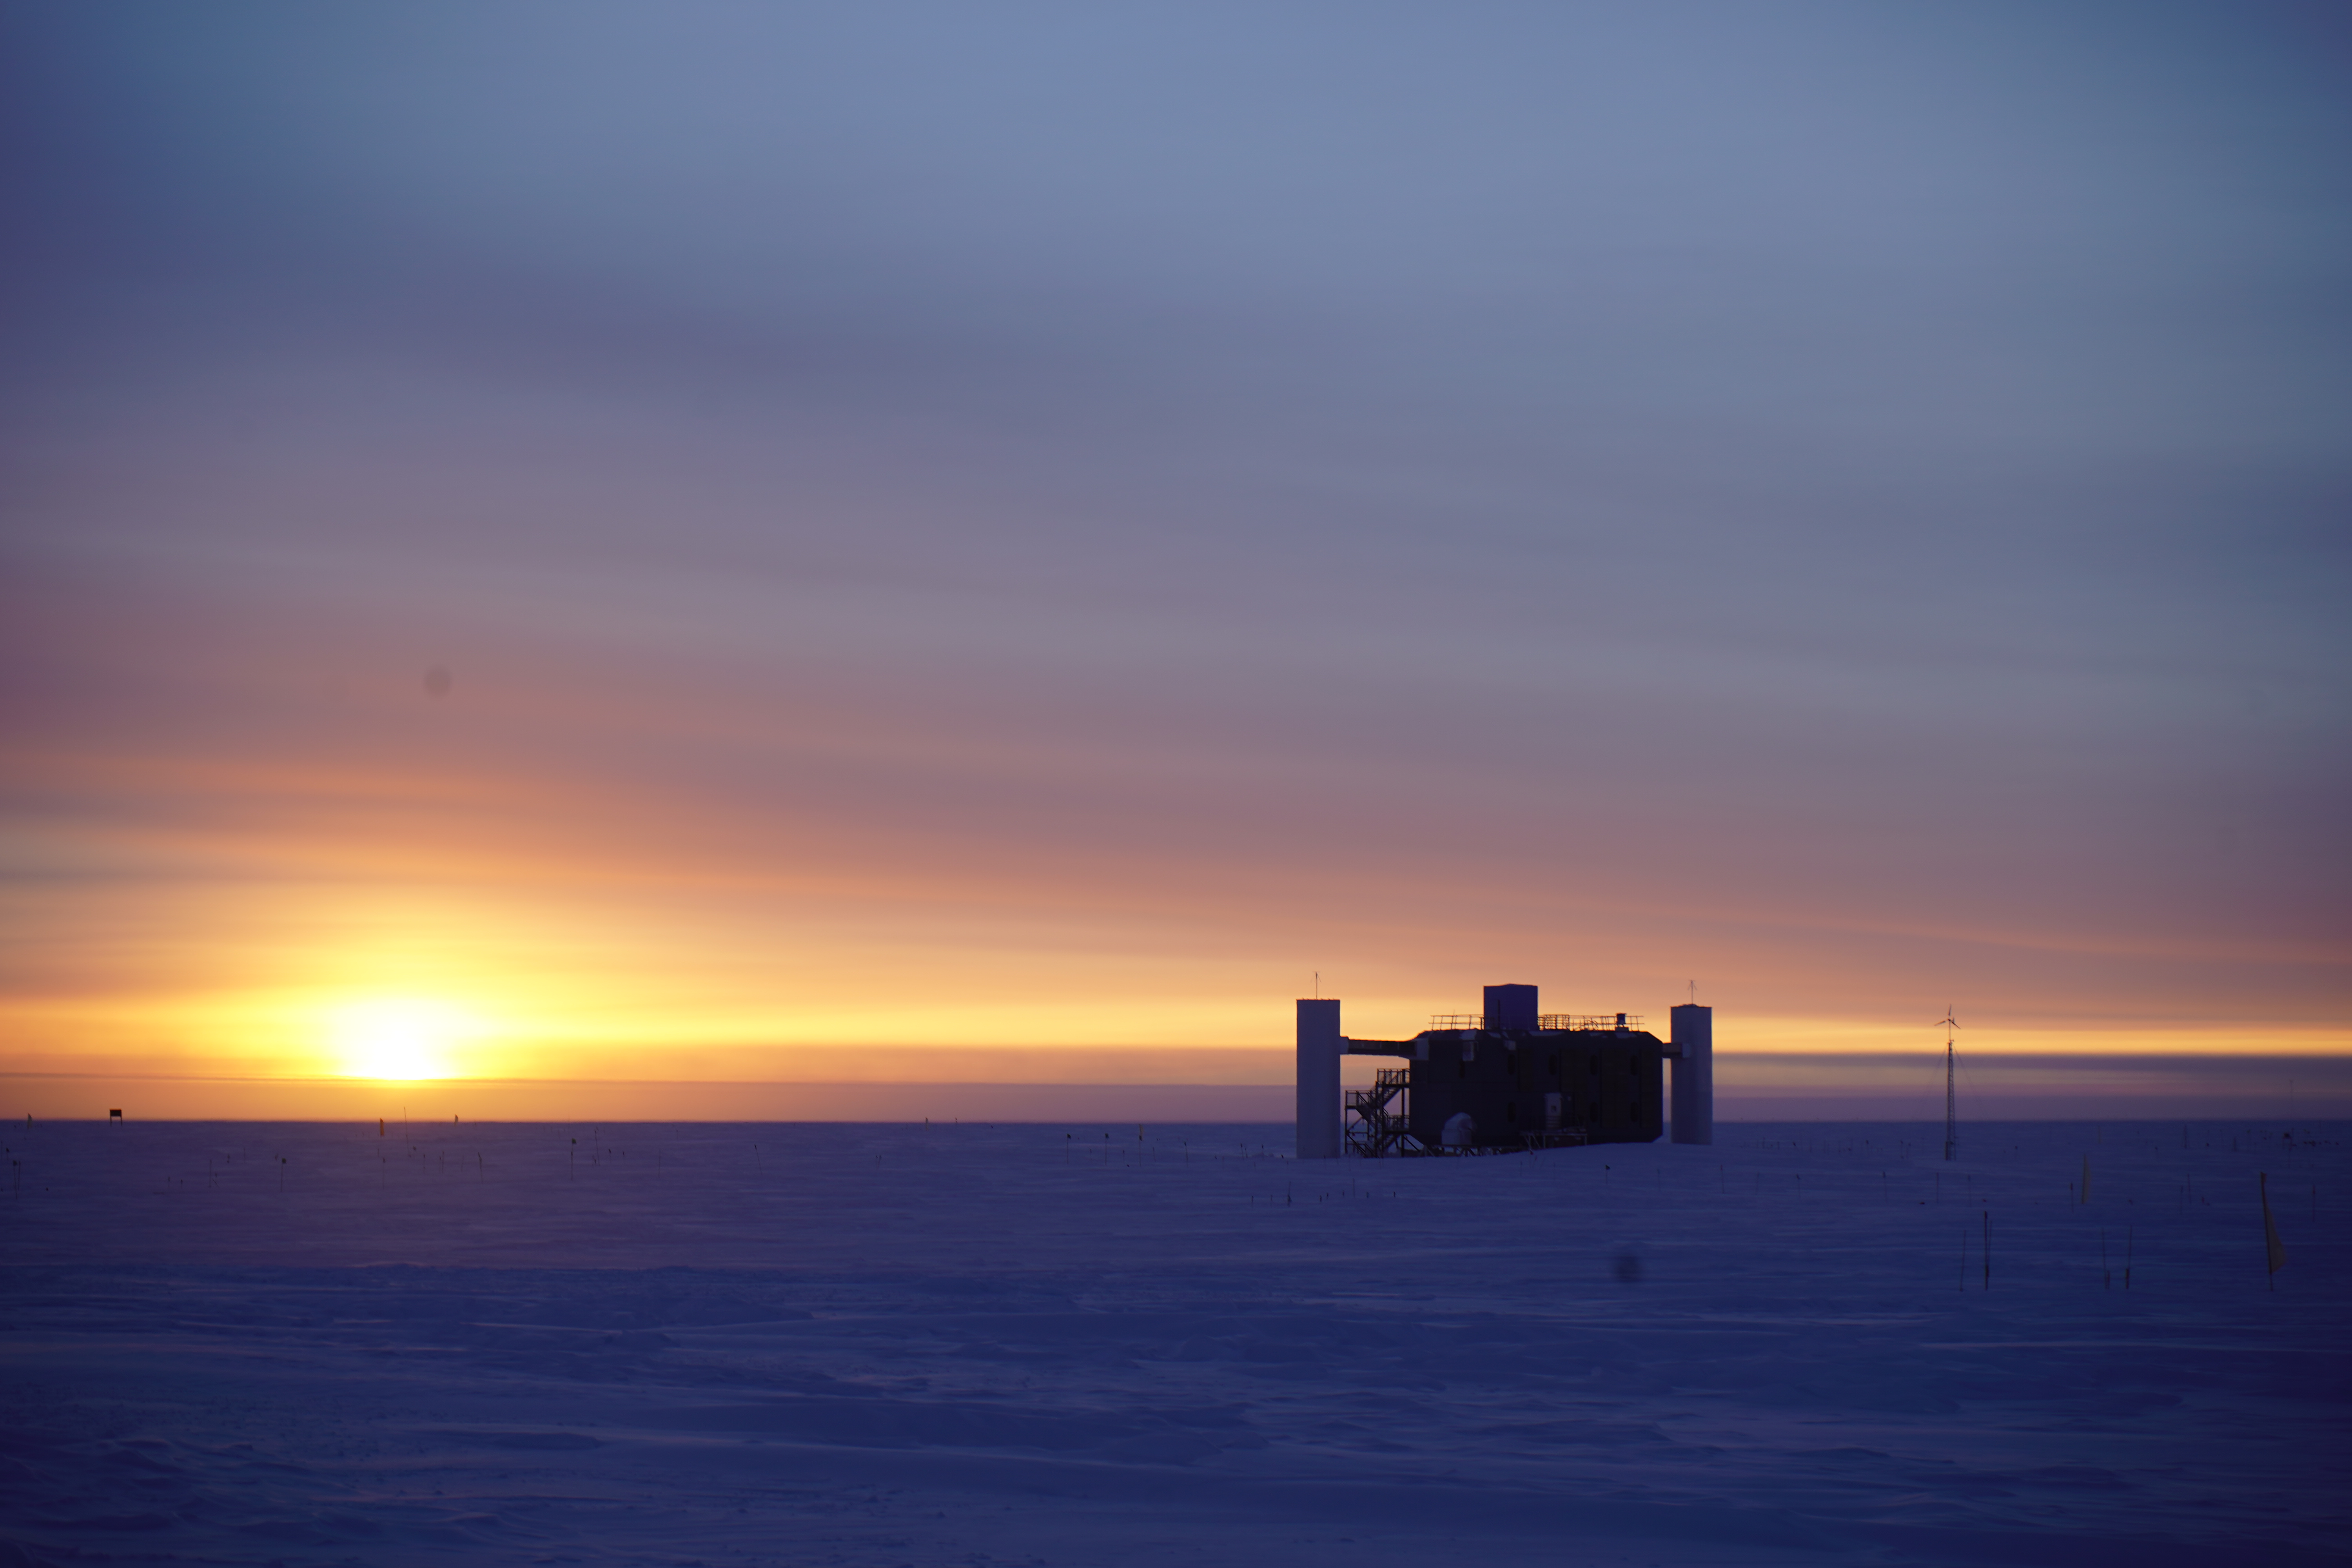
\includegraphics[scale=0.37]{figures/ic3/ICL.JPG}
    }\caption{IceCube Laboratory (ICL) that houses the data acquisition systems. Picture from \cite{IceCube_SPGallery}.}
    \label{fig:ICL}
\end{figure}

\begin{figure}
    \centering{
        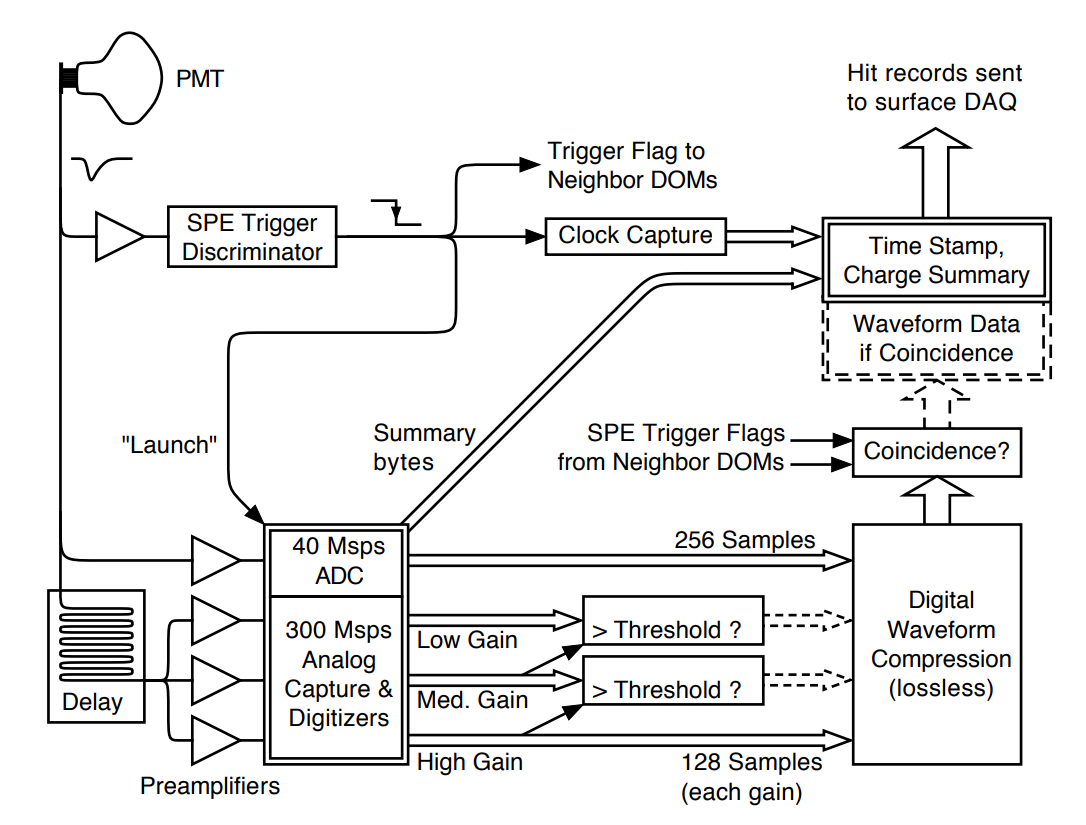
\includegraphics[scale=0.4]{figures/ic3/IC3_dataflow.png}
    }
    \caption{Data flow chart PMT waveforms from the DOMs. “Hit Records" are sent to the surface DAQ computers in ICL. Full waveform data, represented with dashed arrows, are included when neighboring DOMs are hit in coincidence above the SPE discriminator threshold.}
    \label{fig:IC3_dataflow}
\end{figure}

The data acquisition process in IceCube starts when a PMT within a DOM detects light surpassing a threshold of 0.25 photoelectrons.
The importance of the information transmitted to the ICL depends on the detection of hits in neighboring DOMs within a microsecond window.
Isolated signals prompt a Soft Local Coincidence (SLC) response, transmitting only a timestamp and a charge summary.
In contrast, signals detected by neighboring DOMs initiate a Hard Local Coincidence (HLC).
The full waveform is compressed and sent along with the timestamp and charge summary to the ICL \cite{IC3_thedetector}.
\Cref{fig:IC3_dataflow} shows a flow chart of PMT data within the DOMs before being sent to the ICL.

Achieving uniform timing across DOMs is essential for accurate event reconstruction.
Each DOM's independent clock is finely calibrated and synchronized with the ICL's clocks.
Times are translated to Universal Coordinated Time (UTC).
This calibration is set by sending continuous pulses between the DOMs and the ICL.
The waveforms are adjusted by subtracting the common baseline and applying the gain \cite{IC3_thedetector}.

Within the ICL, the Data Acquisition (DAQ) system employs various trigger algorithms to discern neutrino events from the vast majority of DOM hits caused by dark noise.
One such mechanism, the Simple Multiplicity Trigger (SMT), requires a specific number of HLC hits within a brief timeframe to recognize a series of hits as an event \cite{IC3_thedetector}.

Further refining the observatory's data, the Processing and Filtering (PnF) system, also housed within the ICL, applies around 25 different filters after initial event detection.
Each filter is designed for specific physics analyses.
The system employs filters such as: The Muon Track Filter to isolate high-quality track events crucial for neutrino source identification;
the Shower Event Filter to select events with large energy deposits indicative of neutrino interactions;
and the High-Charge Filter to highlight events with extensive photoelectron deposits \cite{IC3_thedetector}.
These filters ensure that the data prepared for further analysis and transmission to researchers in the Northern Hemisphere contains the most significant scientific insights \cite{IC3_thedetector}.

The operational control of the observatory, maintained by the LiveControl system within the ICL, oversees the DAQ and PnF systems.
It handles the initiation and conclusion of data-taking runs and maintains a database of operational parameters.
LiveControl alerts operators to any deviations from expected conditions.
It is crucial for ensuring that the observatory operates within its optimal parameters \cite{IC3_thedetector}.

%-----------------------------------------------------------------------------------%
\section{Event Reconstruction}
%-----------------------------------------------------------------------------------%
Event Reconstruction within the IceCube Neutrino Observatory transforms signals captured by DOMs into quantifiable scientific insights.
The goal of event reconstruction is to ascertain the origin, trajectory, and energy of interacting neutrinos.
This process is pivotal for interpreting signals as either originating from celestial neutrino sources or other phenomena.
I will focus mostly on how IceCube reconstructs track-like events as these are the most relevant for this dissertation.

%$$$$$$$$$$$$$$$$$$$$$$$$$$$$$$$$$$$$$$$$$$$$$$$$$$$$$$$$$$$$$$$$$$$$$$$$$$$$$$$$$$$%
\subsection{Tracks and Cascades}
%$$$$$$$$$$$$$$$$$$$$$$$$$$$$$$$$$$$$$$$$$$$$$$$$$$$$$$$$$$$$$$$$$$$$$$$$$$$$$$$$$$$%

\begin{figure}
    \centering{
        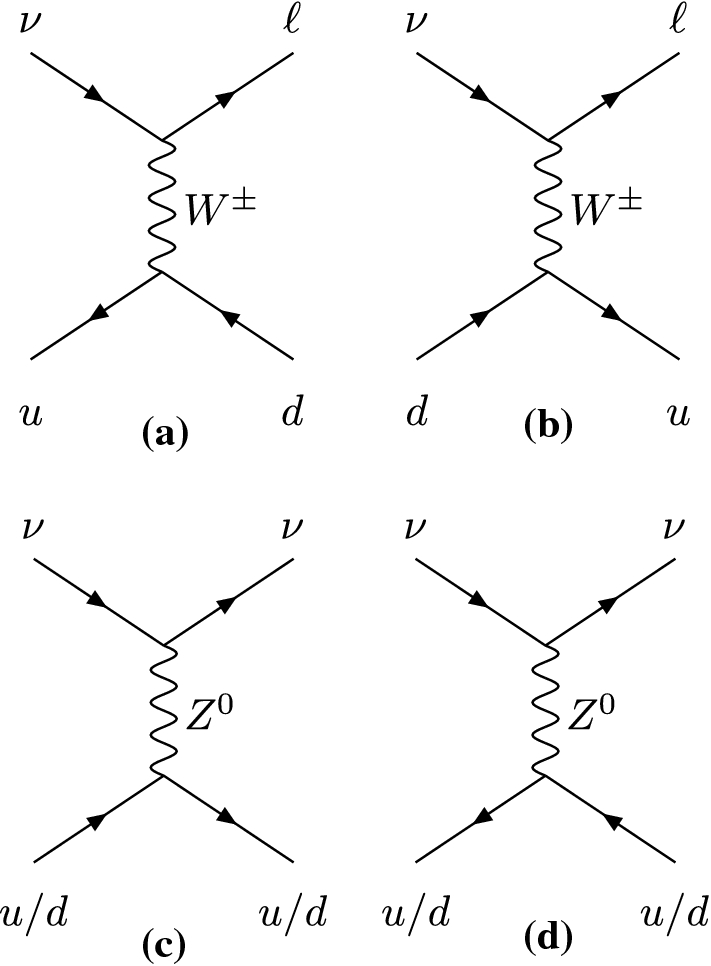
\includegraphics[scale=0.3]{figures/ic3/nn_cc_feynman.png}
    }
    \caption{Feynman diagrams for W (a/b) and Z (c/d) boson mediated interactions between neutrinos and light quarks. Charged current (CC) interactions are shown in panels a and b. Neutral current (NC) interactions are shown in panels c and d. NC interactions occur between neutrinos and quarks within atomic nucluei in the ice. CC interactions will exchange W bosons and produce a lepton corresponding to the neutrino flavor and a hadronic cascade. NC interactions will exchange a Z boson and produce a hadronic cascades. Figure from \cite{physics_withIC3}.}
    \label{fig:ic2_ccORnc}
\end{figure}

\begin{figure}
    \centering{
        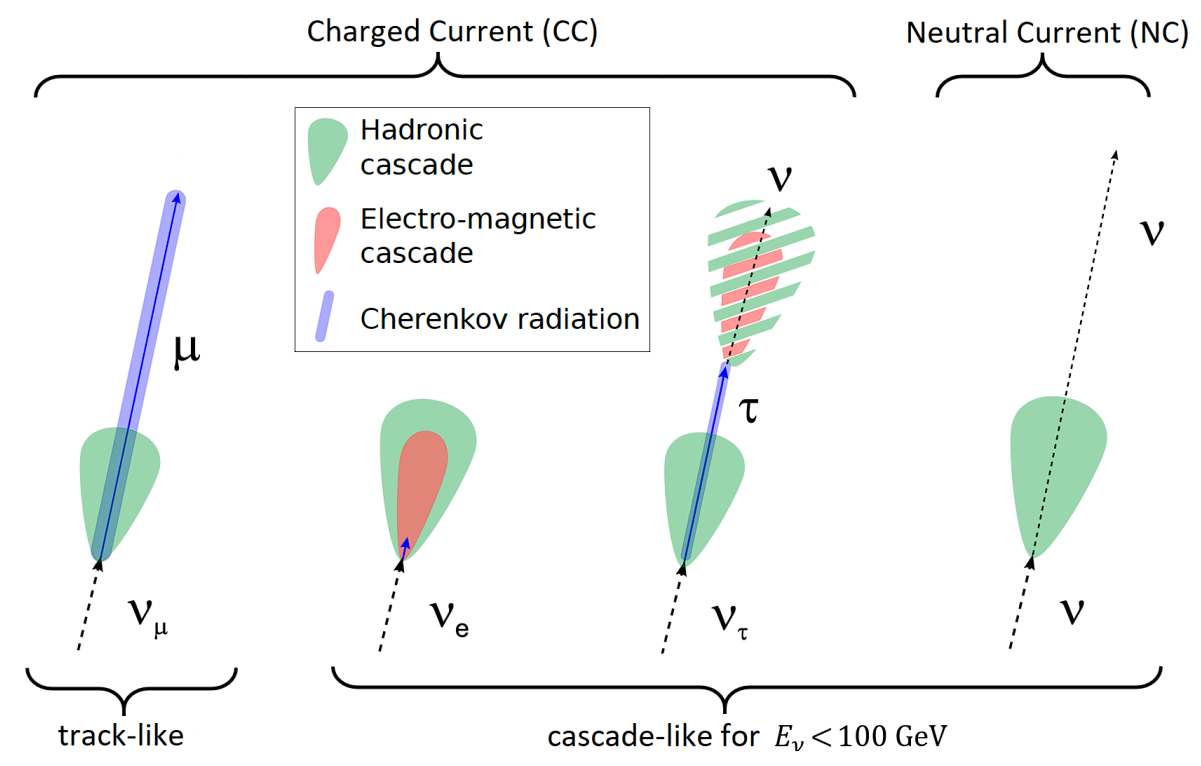
\includegraphics[scale=0.4]{figures/ic3/event_topologies.png}
    }
    \caption{Event topologies for high energy NC and CC neutrino interactions with ice. Signatures can be split as either: hadronic and electromagnetic cascades; Cherenkov radiation from a charged, long-lived particle. Cascades from $\tau$ decays will depend on its decay products. For energies below 1 PeV the double bang of the $\nu_\tau$ signature overlap and are indistinguishable. Figure from \cite{rene_thesis_nutracks}.}
    \label{fig:event_topology}
\end{figure}

\begin{figure}
    \centering{
        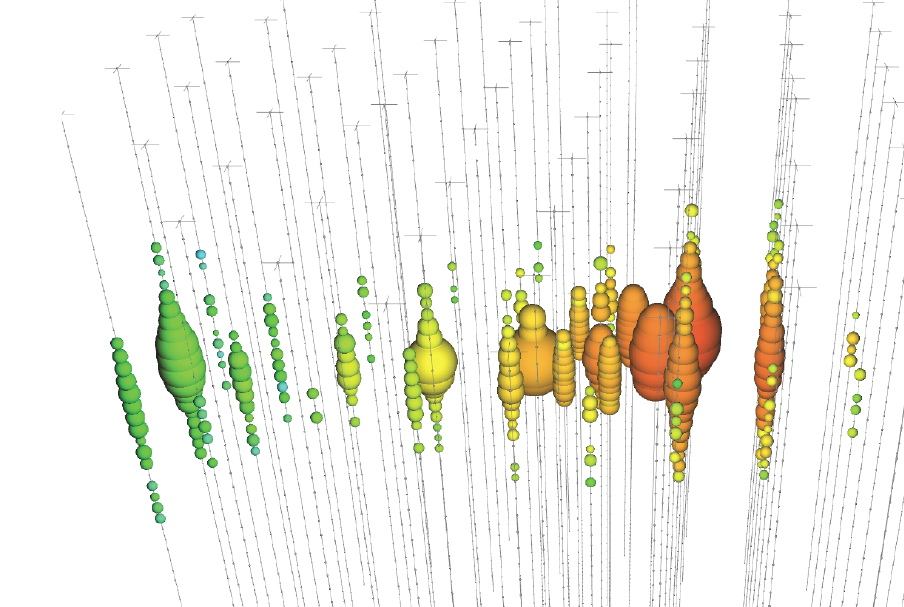
\includegraphics[scale=0.5]{figures/ic3/neutrinos-track-sig-2.png}
    }
    \caption{A simulation of a track-like event in IceCube. Redder bubbles indicate earlier photon arrival times. Greener bubbles occur later. The size of the DOM bubble illustrate the charge deposition in the DOM. For this event, the CC neutrino interaction occurred by the red hits. There is then a long muon track going to the left. Figure taken from \cite{IC3_masterclass}.}
    \label{fig:ic3_track}
\end{figure}

\begin{figure}
    \centering{
        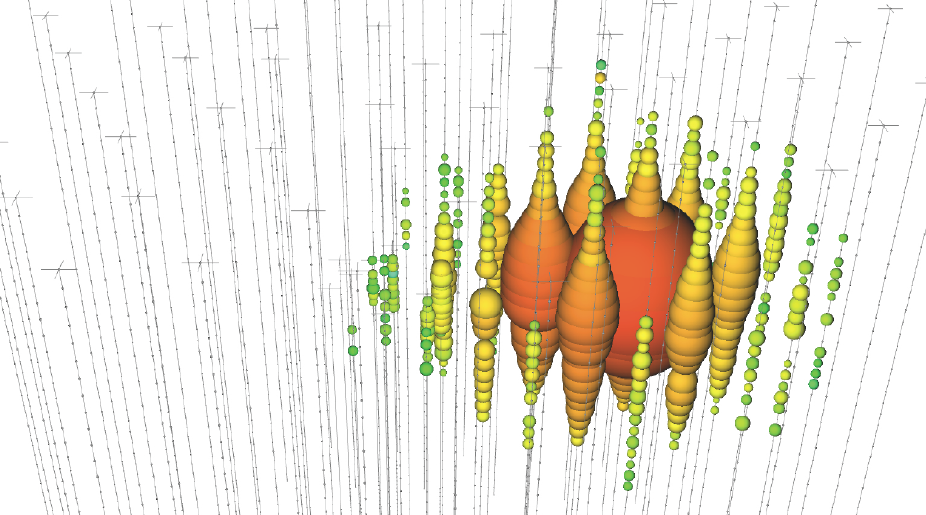
\includegraphics[scale=0.5]{figures/ic3/neutrinos-cascade-sig-1.png}
    }
    \caption{Same as \cref{fig:ic3_track} but for a cascade-like event. Figure taken from \cite{IC3_masterclass}.}
    \label{fig:ic3_cascade}
\end{figure}

\begin{figure}
    \centering{
        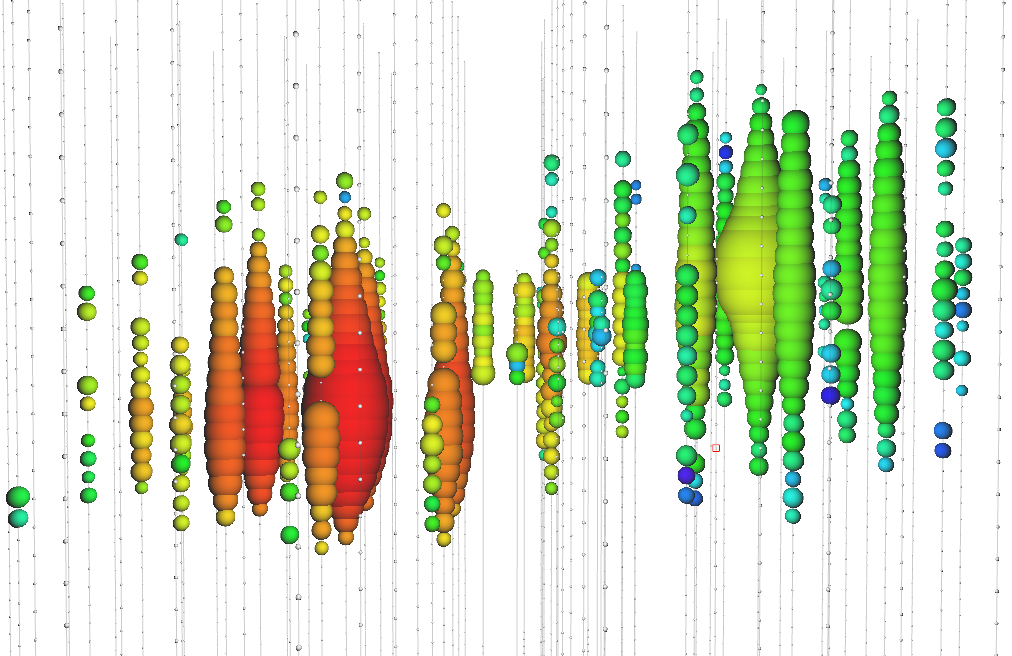
\includegraphics[scale=0.45]{figures/ic3/neutrinos-double-bang-sig-3.png}
    }
    \caption{Same as \cref{fig:ic3_track} but for a double-bang event. Two distinct cascades are visible if the initial neutrino is very high energy. Figure taken from \cite{IC3_masterclass}.}
    \label{fig:ic3_doubleBang}
\end{figure}

Events in IceCube's detector volume manifest primarily as either tracks or cascades.
The primary cause of the event topology are both the neutrino flavor and the nature of the primary neutrino's interaction with the ice.
\Cref{fig:ic2_ccORnc} presents Feynman diagrams of typical neutrino interactions with particles in the ice.
\Cref{fig:event_topology} illustrates the signatures from various topologies of neutrino interactions in the ice.

Tracks emerge from charged-current (CC) interactions involving muon neutrinos ($\nu_\mu$).
These events are characterized by the production of a high-energy muon ($\mu$).
These muons, due to its relatively large mass compared to electrons, can traverse substantial distances through the ice, exceeding kilometers.
These long trajectories are obvious from their continuous, distinct, and elongated track of Cherenkov light in the ice.
See \cref{fig:ic3_track} for a simulated track event.
The angular deviation between the incoming $\nu_\mu$ and the secondary $\mu$ is notably slight, tapering to near 0.3$^\circ$ above TeV energies.
Therefore, $\mu$ tracks closely approximate the primary neutrino's path \cite{physics_withIC3,IC3_energyReco}.
Such precision affords angular resolutions finer than 1$^\circ$ for TeV neutrinos which facilitates the determination of their cosmic origins \cite{physics_withIC3}.

Cascades are products of both neutral-current (NC) interactions across all neutrino flavors and CC interactions involving electron or tau neutrinos, $\nu_e$ and $\nu_\tau$ respectively.
Unlike tracks, cascades result in a more localized burst of Cherenkov radiation.
The burst imprints as a nearly spherical light pattern from the rapid dissipation of energy by the produced particles.
See \cref{fig:ic3_cascade} for a simulated track event.
This diffusion creates a distinct event signature with good energy estimation, but worse directional clarity compared to track events.
The isotropic nature of cascades leads to larger angular uncertainties, typically around 15$^\circ$.
Yet, cascades excel in providing energy measurements, with resolutions reaching as tight as 15\% from the contained nature of the energy deposition \cite{physics_withIC3,IC3_energyReco}.

The double-bang event, posited for $\nu_\tau$ interacting via CC at energies above 1 PeV, would display as two distinct cascades within the detector.
These events start from an initial interaction and subsequent decay of the $\tau$ lepton over a discernible distance.
See \cref{fig:ic3_doubleBang} for a simulated track event.
The double-bang offers a unique marker for high-energy $\nu_\tau$ detection \cite{physics_withIC3}.
Preliminary whispers of double-bang events IceCube have been observed \cite{IC3_taus}.
Yet, efforts are ongoing to isolate such an event.

%$$$$$$$$$$$$$$$$$$$$$$$$$$$$$$$$$$$$$$$$$$$$$$$$$$$$$$$$$$$$$$$$$$$$$$$$$$$$$$$$$$$%
\subsection{Reconstruction of Track Direction}
%$$$$$$$$$$$$$$$$$$$$$$$$$$$$$$$$$$$$$$$$$$$$$$$$$$$$$$$$$$$$$$$$$$$$$$$$$$$$$$$$$$$%

Angular reconstruction for $\nu_\mu$ induced tracks in the IceCube detector volume starts with the LineFit algorithm \cite{AMANDA_trackreco}.
LineFit estimates the $\mu$'s trajectory through the least squares fit to the Cherenkov light hits on the DOMs.
LineFit assumes the muon propagates with constant velocity and treats its path as linear in order to simplify the emission patterns of Cherenkov radiation.
To improve this approximation, the Huber penalty function \cite{Huber:1964} is applied which distinguishes between signal and noise by considering the spatial distribution of hits relative to the track \cite{IC3_Calibration}.

The reconstruction process is refined further by the Single Photoelectron (SPE) likelihood method, which calculates the probability of photon arrival times at the DOMs \cite{Huber:1964}.
It does so by taking into account the earliest detected photons as they are least likely to have been scattered in the ice:
\spe
where $N_{\mathrm{DOM}}$ is the number of DOMs involved in the event.
$N_{\mathrm{hit}}$ is the number of hits registered \cite{AMANDA_trackreco}.
$p_j(t_i)$ is the probability density function (PDF) of the photon arrival time.
The charge detected by each DOM, $q_i$, factors into the probability calculation, assuming that earlier photons provide more reliable directional information.

An alternative to SPE, the Multi-Photoelectron (MPE) likelihood method accounts for all detected photons.
MPE uses the total observed charge to weight the significance of each hit:
\mpe
where $Q_j$ is the sum of charges observed by the j-th DOM, providing a more detailed picture of the $\mu$'s path \cite{AMANDA_trackreco}.

SplineMPE, is the final step and employs a spline-based parameterization of the photon arrival times.
These spline fits encode a detailed understanding of the ice's optical properties derived from calibration data \cite{AMANDA_trackreco}.
This approach yields the following likelihood function for improved angular resolution:
\splineMPE
where the parameters $\vec{r_0}, t_0, \theta, \mathrm{ and}~\phi$ describe the reconstructed track within IceCube's voluminous array \cite{AMANDA_trackreco}.

From the light weight LineFit to the complex SplineMPE, each step incorporates more detailed physics to enhance the reconstruction's accuracy.
Each hones in on the $\mu$ track to reveal the $\mu$'s cosmic origin.
This multi-stepped tracking is crucial for IceCube's mission to map the universe through the lens of high-energy neutrino interactions.

%$$$$$$$$$$$$$$$$$$$$$$$$$$$$$$$$$$$$$$$$$$$$$$$$$$$$$$$$$$$$$$$$$$$$$$$$$$$$$$$$$$$%
\subsection{Energy}
%$$$$$$$$$$$$$$$$$$$$$$$$$$$$$$$$$$$$$$$$$$$$$$$$$$$$$$$$$$$$$$$$$$$$$$$$$$$$$$$$$$$%

After pinpointing the $\mu$ track's direction, IceCube employs the MuEX algorithm to estimate the energy deposited by the muon inside the detector.
The MuEX algorithm uses a Poisson likelihood model, comparing the observed photoelectrons $k$ to the expected light output, $\Lambda$, which is directly related to the deposited energy $E$:
\muEXLLH
$\rho$ is the number of expected noise photons, and $\Lambda$ reflects the light yield per unit energy, taking into account the optical properties of the ice and the detector response.
The logarithm of the likelihood is minimized with respect to the energy, resulting in a best-fit estimate \cite{IC3_energyReco}.

For a more detailed energy reconstruction, the Millipede algorithm unfolds the muon's energy loss along its path by adapting the Poisson likelihood.
This approach accounts for the stochastic energy losses due to Bremsstrahlung and pair production, treating the $\mu$ as a series of electromagnetic cascades:
\vecMULLH
where $k$ denotes the observed photons, $\rho$ the noise, $E$ the energy losses, and \textbf{$\Lambda$} the matrix of predicted light yields throughout the detector.
By fitting the muon's position, direction, and the vector of energy losses, Millipede achieves a resolution on total deposited energy along the muon track of approximately 10-15\% \cite{IC3_energyReco}.

IceCube makes some approximations when estimating $\lambda$ for the reduction of computational time.
Two important assumptions IceCube makes are that Cherenkov light from cascades is spherically symmetric along the $\mu$ track and the Cherenkov emission is uniform \cite{IC3_energyReco}.
The uncertainties in these approximations is accounted for by convolving $\lambda$ with a PDF, $G$, on the light yield.
The likelihood is then rewritten as:
\LLHwithspice
The full description for the PDF, $G(\lambda_i, \lambda_j)$ is discussed in \cite{IC3_energyReco}.
After considering the uncertainties, the energy resolution was observed to be in the range of 30\%-35\% \cite{IC3_energyReco}.

%-----------------------------------------------------------------------------------%
\section{Background}
%-----------------------------------------------------------------------------------%

In IceCube, the primary challenge in detecting astrophysical neutrinos is the background noise from atmospheric neutrinos.
These are produced from cosmic rays hitting the Earth's atmosphere, leading to a cascade that includes both neutrinos and muons (see \cref{fig:airshowers}).
These particles sometimes generate detector signals similar to those from astrophysical sources.

IceCube employs selective criteria to reduce this background.
For instance, downward-moving tracks are scrutinized more heavily, as these are more likely to be related to atmospheric events.
Upward-moving neutrinos, however, are less likely to be confused with this background because the Earth filters out most other particles, including muons.
The detector uses the Earth itself as a filter to increase the purity of potential astrophysical neutrino signals.
This differentiation between upgoing and downgoing events helps IceCube focus on the neutrinos that are of most interest for astronomical observations.